\chapter{Anatomy of Information Transfers during Earnings Season}

Using Transfer Entropy (TE), a measure from information theory, we detect sub-minute, directed information flows across prices between firms in the S\&P 500 in Q1 2018. We examine the structural properties of TE between firms. 

Then TE is used to predict future price direction with machine learning models. Overall the results show that TE is useful predictor for predicting future price changes. 

\section{Introduction}

Prior studies (i.e \cite{}) have examined price changes over long (monthly, daily, or hourly) windows and relatively short windows (minutes). However much of the price change process may have not have been captured during these windows given that information is reflected in price within seconds. We proposed an alternative methodology to measure and capture more of the information transfer process between firms in the S\&P 500 using measures from information theory (see \ref{sec:}). We then employ machine learning models to predict short-term price change using information transfers between firms.

For the remainder of the paper, we discuss the dataset used to estimate TE. The methodology of estimating information transfers is described followed by a description of the properties of the estimates. We then employ network science to observe the patterns and structural properties of the estimates. We then employ several machine learning models to predict short-term price change using network metrics from the information transfer. The results are discussed in addition to future directions that this research can take.

\section{Data}
\label{sec:Data}

The data in the study comes from Wharton Research Data Services (WRDS).  Security prices are obtained from the trade and quote (TAQ) dataset which contains all trades and quotes that occurred at a sub-second level. The national best bid/offer (NBBO) price is determined by the lowest ask price and highest bid price available from multiple exchanges. The NBBO prices are identified from the TAQ dataset and are sampled at a particular rate.  The NBBO price data is obtained for firms in the S\&P 500 in Q1 2018.  Ten datasets are constructed for each firm at different sampling rates. The sampling rates used are $1$ second, $2$ seconds, $3$ seconds, $4$ seconds, $5$ seconds, $10$ seconds, $15$ seconds, $30$ seconds, $60$ seconds, and $120$ seconds. For example at $1$ second sampling rate there will be 120 NBBO price observations per minute for a particular firm.

Also IBES data
Also Compustat data?

\subsection{Estimating Information Flow}

TE is used to estimate the amount of information flow between every unique pair of firms in the S\&P 500 during Q1 2018 (the first 61 days of 2018). To detect information flow at the minute/sub-minute level between firms in the S\&P 500, first the NBBO prices will be obtained from the TAQ data for all firms in the S\&P 500 in Q1 2018. For each date and firm from the NBBO data I will create 10 datasets for that particular date and firm which samples the NBBO price data with the following sampling rates: 1, 2, 3, 5, 6, 10, 30, 60, and 120 seconds.

The idea behind sampling the NBBO price data is to help determine at what speed is information transfer between firms the strongest, weakest, or most persistent. Next for each date, firm, and sampling rate bi-variate TE will be estimated with the NBBO sampled price data using three 130 minute intervals throughout the trading day; the rationale behind this is to determine if there are any consistent information flow patterns during the beginning (9:30am-11:40am), middle (11:40am-1:50pm), or end (1:50pm-4pm) of the trading day. To summarize TE will be estimated to the current firm from all other firms in the S\&P 500 for that particular date, sampling rate, and interval. Given that there are 10 sampling rates, 3 intervals, 61 days, and theoretically 499 other firms, this amounts to 913,170 TE calculations per firm for Q1 2018. This same process will be repeated for 30 minute windows (i.e 9:30am-10am, 10am-10:30am, ..., 3:30pm-4pm) which yields 3,957,070 calculations. 

Small sample rates will yield a high number of observations to estimate TE with. Given that open source implements were not suited to estimate bi-variate TE on big data (see Chapter \ref{Chapter:PyIF} we utlize PyIF (see \cite{PyIF}). Currently TE estimates are computed using the HAL cluster at the National Center for Supercomputing Applications using a single NVIDIA V100 GPU. The 1 second sampling rate has the most observations and is the most costly to estimate TE. For a particular day, TE computations on HAL to 1 firm from the other 499 firms for the 3 intervals will take \textbf{N} minutes. For all 500 firms this would take \textbf{N*500}. For all days in Q1 2018, this would take \textbf{N*500*61} at the 1 second sampling rate. Subsequently for the 2 second sampling rate the data is reduced by 2 and it takes \textbf{(N*500*61)/2} blah to estimate TE between all firms.

\subsubsection{Algorithmic Process for Estimating Information Flows Between firms}

In this section the algorithmic process is outlined to estimate information transfer between firms using the Q1 2018 data (see Algorithm \ref{alg:EstIF}). In Algorithm \ref{alg:EstIF} Given sampling rates in line 2 and dates of interest  in line 1 we iterate through each date in line 3. For a particular date we iterate through each sampling rate in line 4. For each unique combination of date and sampling rate we select firms with observations in that date and sampling rate. We then create an empty matrix of size Firms\(_i\))\(^2\) by 3.  Then we create a counter variable to keep track of the observations in line 8. 

Next we iterate through each firm in the set of firms\(_i\).  In algorithm \ref{alg:EstIF} the trading day is split 3 into 2 hour and 10 minute windows which represents the beginning (9:30am-11:40am),  middle (11:40am-1:50pm),  and end of the trading day (1:50pm-4pm).  In lines 10-12 we filter the NBBO prices for firm i to the beginning of the trading day,  middle of the trading day, and end of the trading day.  For a single firm from the set of firm\(_i\). We repeat this process for all of the firms in the set firm\(_j\) We then estimate Transfer Entropy from firm\(_j\) to firm\(i\)  and assign the TE estimate to cnt\(\{_ij\}\). We then increment cnt\(_{ij}\) by 1.  We repeat this algorithmic process with modifications to window size, where we compute TE between firms using 30 minute windows.\\

\begin{algorithm}[H]
\SetAlgoLined
\KwResult{Write here the result }

Dates := All Dates in Q1 2018 \;
SampleRates := [1, 2, 3, 4, 5, 6, 10, 30, 60, 120] secs \;

\For{\(t \in \) Dates}{
	\For{\(SR \in \) SampleRates}{
		Firms\(_i \) := SelectFirms(\(t,SR\)) \;
		Firms\(_j \) := SelectFirms(\(t,SR\)) \;
		dateSR\_InfoFlow := Matrix(length(Firms\(_i\))\(^2\), 3) \;
		cnt\(_{ij}\): = 0 \;
		\For{Firm\(_i \in\) Firms\(_i\)}{
			MoPrices\(_i\) := Filter(Firm\(_i\), “9:30am-11:40am”) \;
			MidPrices\(_i\) := Filter(Firm\(_i\), “11:40am-1:50pm”) \;
			AfterPrices\(_i\) := Filter(Firm\(_i\), “1:50pm-4:00pm”) \;	
						
			\For{Firm\(_j \in\) Firms\(_j\)}{
				MoPrices\(_j\) := Filter(Firm\(_j\), “9:30am-11:40am”) \;
				MidPrices\(_j\) := Filter(Firm\(_j\), “11:40am-1:50pm”) \;
				AfterPrices\(_j\) := Filter(Firm\(_j\), “1:50pm-4:00pm”) \;
				
				dateSR\_InfoFlow[cnt\(_{ij}\),0] := ComputeTE(MoPrices\(_i\), MoPrices\(_j\)) \;
				dateSR\_InfoFlow[cnt\(_{ij}\),1] := ComputeTE(MidPrices\(_i\), MidPrices\(_j\)) \;
				dateSR\_InfoFlow[cnt\(_{ij}\),2] := ComputeTE(AfterPrices\(_i\), AfterPrices\(_j\)) \;
				
				cnt\(_{ij}\) += 1
			}
		}
	}
}

\caption{Estimating Information Flows Between Firms}
\label{alg:EstIF}
\end{algorithm}

\subsection{Network Creation}

After all bi-variate TE estimates are computed exploratory data analysis will be conducted to find patterns or interesting characteristics of the information transfer between firms to further explore.   First, network analysis (see Chapter \ref{sec:NetworkScience}) will be performed by creating a network for all firms at date $t$, sampling rate $s$, and interval $i$. The nodes for each network will be the firms at $t,s,i$ with edges that have a weight determined by TE.  The process of creating networks where $t=61$ days,  $s=10$ sampling rates, and $i=3$ 2 hour and 10 minute windows will produce roughly 1,830 networks which will make it difficult to discover general insights from the data. When $i=13$ 30 minute windows this will produce 7,930 networks.  

Given that the Kraskov estimator has a downward bias (see Chapter \ref{IFinFM}) some TE values are slightly below 0.  Figures \ref{fig:20180102-1sec-1of3},  \ref{fig:20180102-1sec-2of3},  and \ref{fig:20180102-1sec-3of3},  show examples of a reduced network on January 2nd 2018 at the 1 second sampling rate between 9:30am-11:40am, 11:40am-1:50pm, and 1:50pm-4pm respectively.   Each of these figures show a portion of the firms in the S\&P 500 and the connections between them, where the firms are the nodes and the connections are the edges with a thickness determined by the value of the transfer entropy estimate.  The highest 0.5\% of edges in the network at these particular times are displayed.  

The node size represents how many connections a firm has between a window.  For all 3 figures roughly 2000 edges are displayed, displaying the full 250,000 connections would yield a network where the ratio of firms to connections is too high to display in this display.  Nevertheless,  representing the data as a network offers an alternative strategy which allows us to compute common network metrics and explore the relationships between firms.

\section{Exploratory Data Analysis}

Tables 1A
Table 1B 
Table 1B 30 minute windows
Table 2
Table 2a
Table 2b
Table 3
Table 4
Table 5

We begin by examining the distributions of the Transfer Entropy estimates per sampling rate computed at 2 hour and 10 minute windows and 30 minute windows.  Figure \ref{fig:130MinDist} and \ref{fig:30MinDist} show  the TE distributions at 2 hour and 10 minute windows and 30 minute windows respectively.  Given that the kraskov estimator has a downward bias both of these distributions provide evidence that there's information flowing between many firms in the S\&P 500.

For both sets of distributions as the sampling rate increases the variance of the TE values increase.  More TE values have a negative information transfer (meaning little to no information transfer is occurring) at higher sampling rates.  The amount of observations used for each TE computation is a potential explanation for the increase in variance.  As the same rate increases we have less observations to estimate Transfer Entropy with. Table \ref{tab:WindowLength} shows the number of observations used for a single firm at a particular sampling rate and window.

The weighted in-degree and out-degree centralities were computed using networks for each window and sampling rates.  Figure \ref{fig:130MinDist-OutDeg}  shows the distribution of weighted in-degree centralities for the 130 minute windows.  As the sampling rate increases the amount of firms that have a lower centrality increases.  To state this differently as the sampling rate increases more firms become less central or important in a network.  Figure \ref{fig:130MinDist-InDeg} shows the distribution of weighted out-degree centralities which do not have a similar patterns across sample rates.  The distributions remain similar to each other with a slight change in mean and variance. 

A similar effect occurs for the distribution of weighted out-degree and in-degree centralities with 30 minute window networks (see figures \ref{fig:30MinDist-InDeg} and \ref{fig:30MinDist-OutDeg}.  Incoming Information Transfers tend not to be central (or important) with respect to other firms in the S \&P 500 at higher sampling rates.  This could indicate that more meaningful incoming information transfers to a firm are captured more at lower sampling rates.   Given these findings from the exploratory data analysis we explore the utility of these network measures for trading strategies.


\section{Information Transfer Attribute to Earnings news}



\section{Predicting Price Change with Information Transfer}
We use Logistic Regression, 

RFC


\section{Results}
foo


\section{Future Work}
More data can lead to more promising results.

\section{Figures and Tables}

\subsection{Figures}
\begin{figure}[!htb]
  \centerline{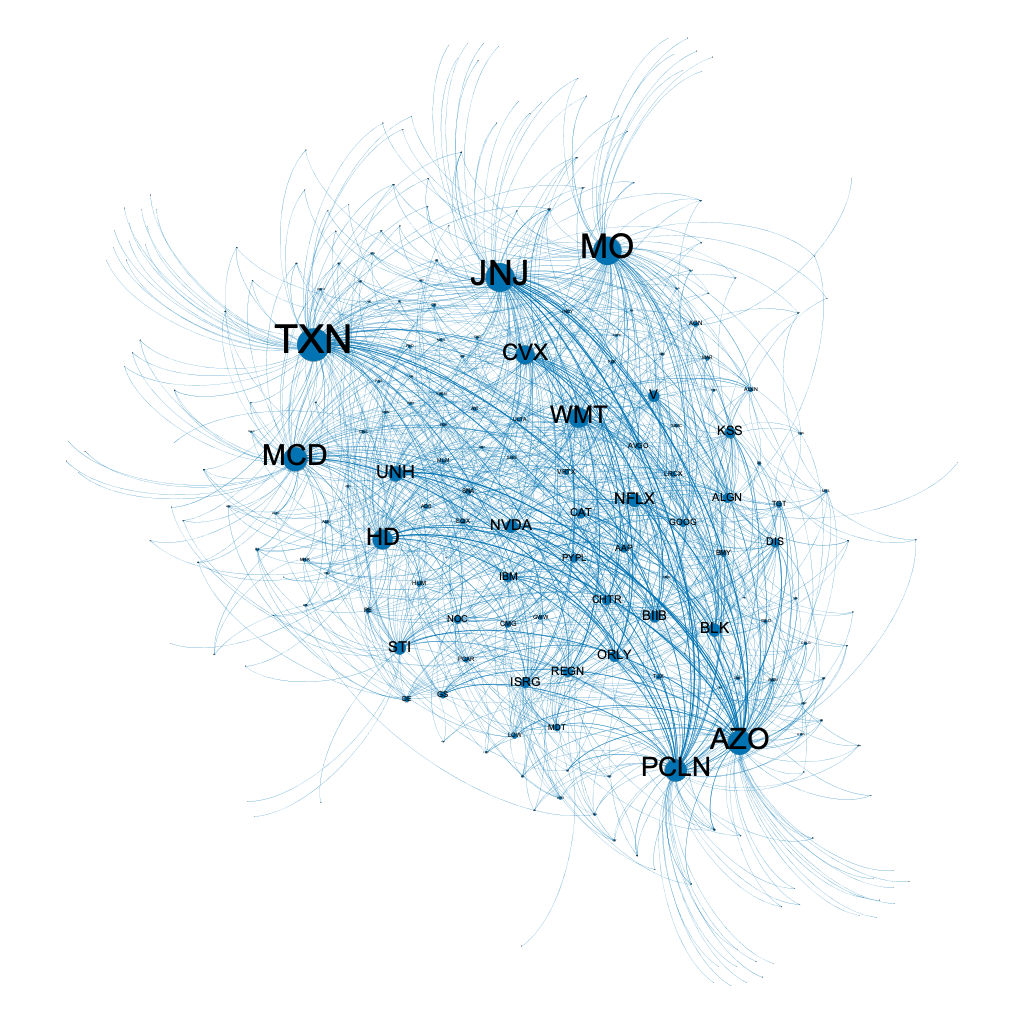
\includegraphics[scale=0.6]{figures/PredIF/Networks/figures/20180102-1sec-1of3.png}}
  \caption{Transfer Entropy Network for firms in the S\&P 500 during January 2nd 2018 between 9:30am-11:40am. }
  \label{fig:20180102-1sec-1of3}
\end{figure}

\begin{figure}[!htb]
  \centerline{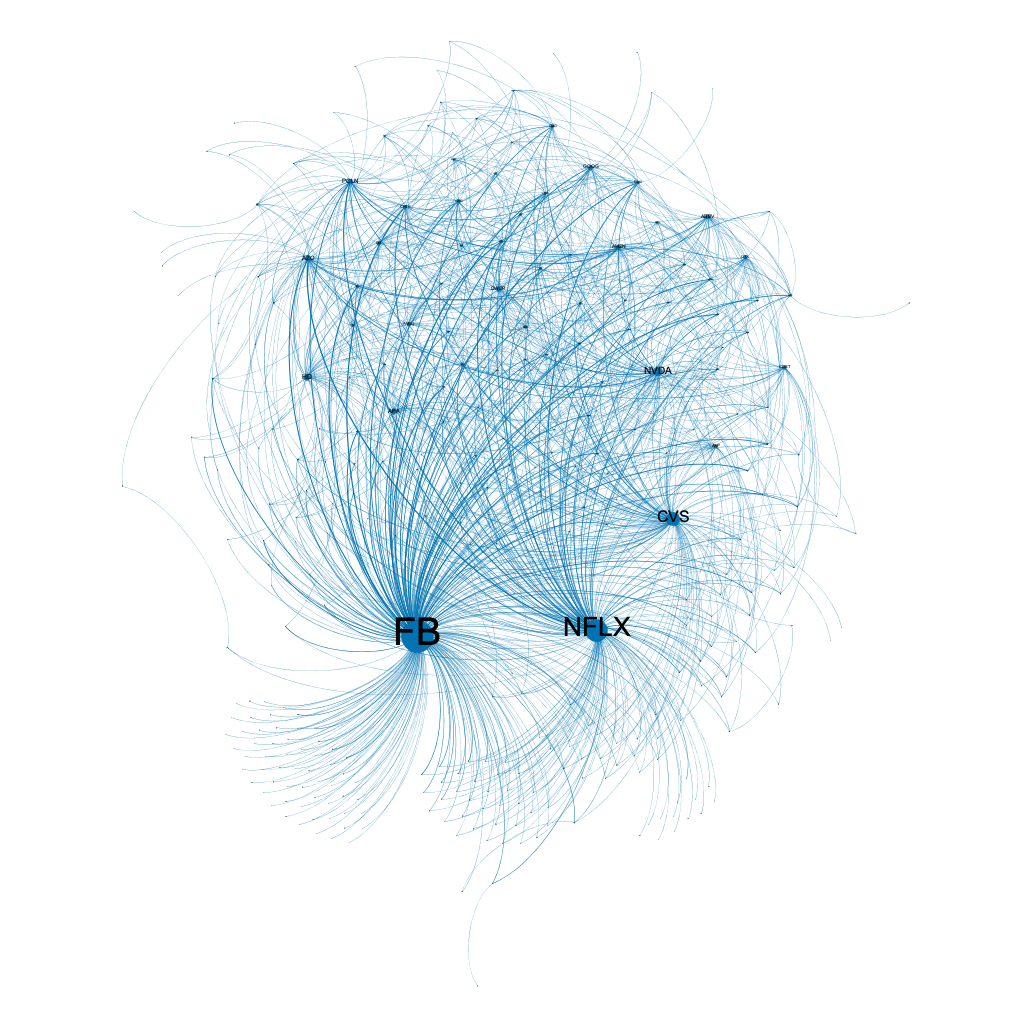
\includegraphics[scale=0.6]{figures/PredIF/Networks/figures/20180102-1sec-2of3.png}}
  \caption{Transfer Entropy Network for firms in the S\&P 500 during January 2nd 2018 between 11:40am-1:50pm. }
  \label{fig:20180102-1sec-2of3}
\end{figure}

\begin{figure}[!htb]
  \centerline{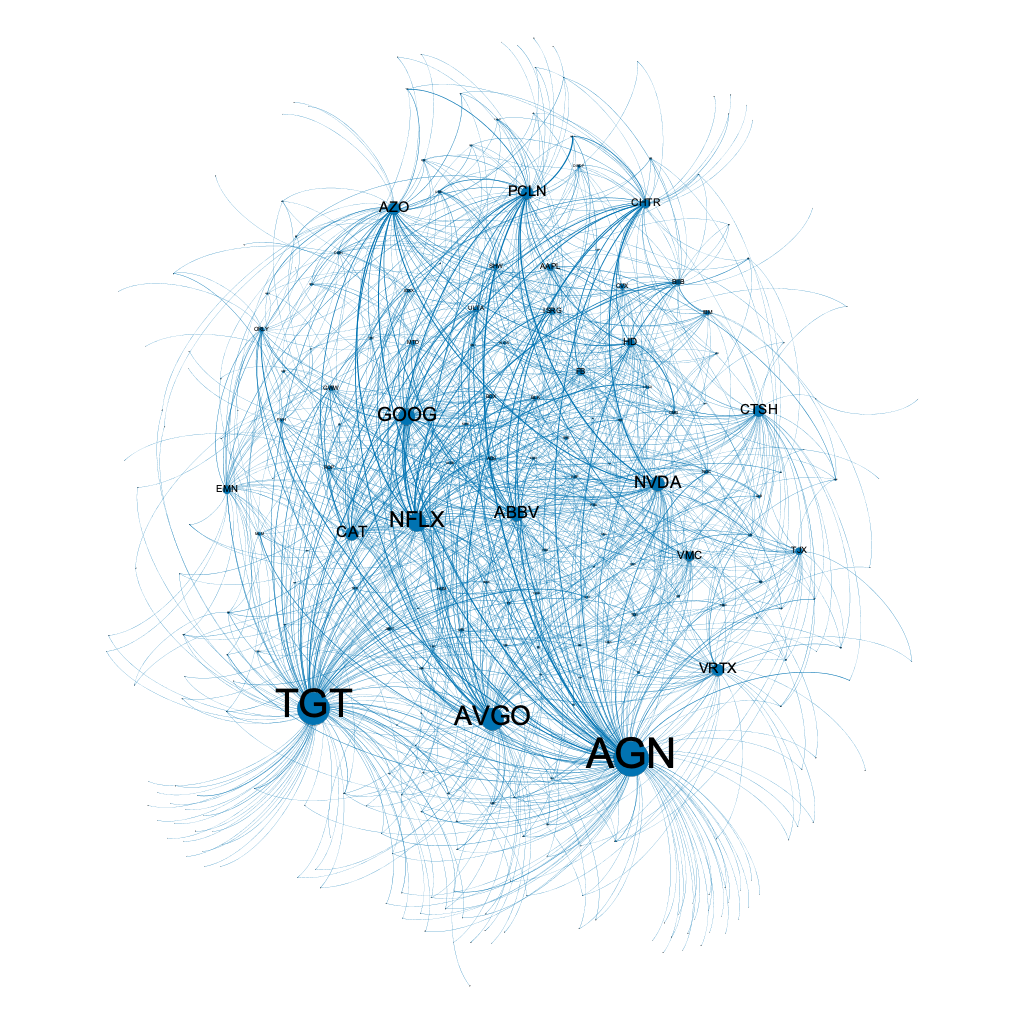
\includegraphics[scale=0.6]{figures/PredIF/Networks/figures/20180102-1sec-3of3.png}}
  \caption{Transfer Entropy Network for firms in the S\&P 500 during January 2nd 2018 between 1:50pm-4:00pm. }
  \label{fig:20180102-1sec-3of3}
\end{figure}

\begin{figure}[!htb]
  \centerline{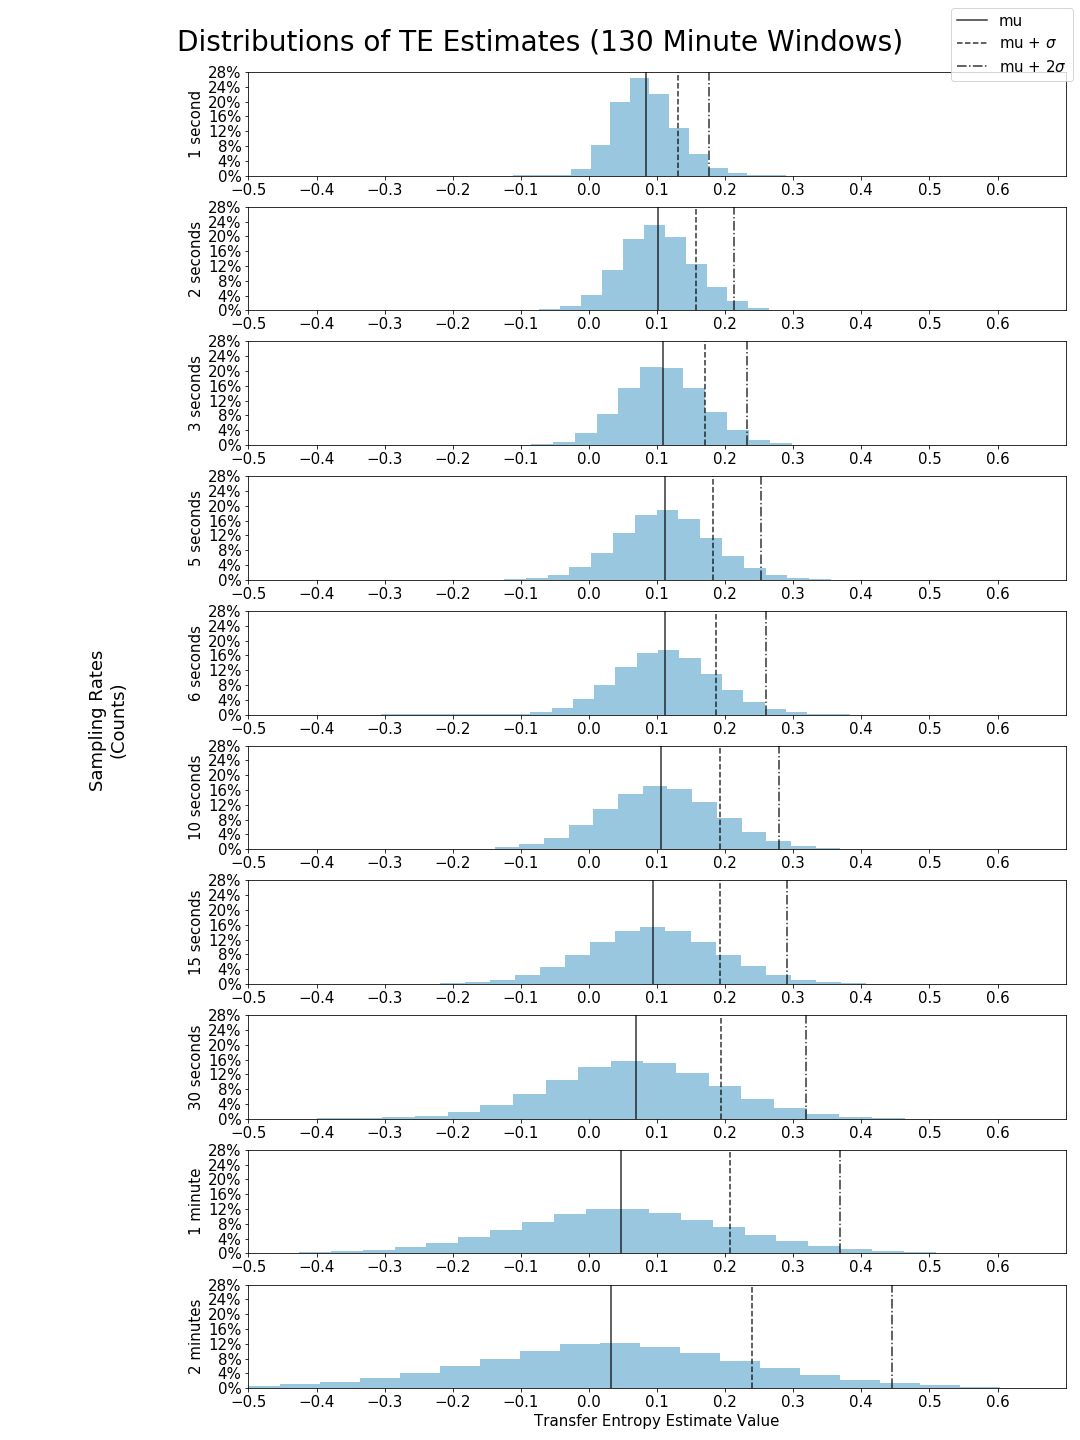
\includegraphics[scale=0.42]{figures/PredIF/130MinDist.png}}
  \caption{Shows the distribution of TE estimates computed with 2 hour and 10 minutes (or 130 minute) windows at various sampling rates.}
  \label{fig:130MinDist}
\end{figure}

\begin{figure}[!htb]
  \centerline{\includegraphics[scale=0.42]{figures/PredIF/30MinDist.png}}
  \caption{Shows the distribution of TE estimates computed with 30 minute windows at various sampling rates.}
  \label{fig:30MinDist}
\end{figure}

\begin{figure}[!htb]
  \centerline{\includegraphics[scale=0.42]{figures/PredIF/130MinDist-InDeg.png}}
  \caption{Shows the distribution of In-Degree Centralities computed with 2 hour and 10 minutes windows (or 130 minute) networks at various sampling rates.}
  \label{fig:130MinDist-InDeg}
\end{figure}

\begin{figure}[!htb]
  \centerline{\includegraphics[scale=0.42]{figures/PredIF/130MinDist-OutDeg.png}}
  \caption{Shows the distribution of Out-Degree Centralities computed with 2 hour and 10 minutes  windows(or 130 minute) networks at various sampling rates.}
  \label{fig:130MinDist-OutDeg}
\end{figure}

\begin{figure}[!htb]
  \centerline{\includegraphics[scale=0.42]{figures/PredIF/30MinDist-InDeg.png}}
  \caption{Shows the distribution of In-Degree Centralities computed with 30 minute windows networks at various sampling rates.}
  \label{fig:30MinDist-InDeg}
\end{figure}

\begin{figure}[!htb]
  \centerline{\includegraphics[scale=0.42]{figures/PredIF/30MinDist-OutDeg.png}}
  \caption{Shows the distribution of Out-Degree Centralities computed with 30 minute windows networks at various sampling rates.}
  \label{fig:30MinDist-OutDeg}
\end{figure}

\newpage
\subsection{Tables}

\begin{table}[!htb]
\centering
\begin{tabular}{c|c|c|}
\cline{2-3}
\textbf{}                                      & \multicolumn{2}{c|}{\textbf{Window Length (in minutes)}}                 \\ \cline{2-3} 
\multirow{2}{*}{\textbf{}}                     & \multirow{3}{*}{{\textbf{130}}} & \multirow{3}{*}{{\textbf{30}}} \\
                                               &                                     &                                    \\ \cline{1-1}
\multicolumn{1}{|l|}{\textbf{Sample Rate (in seconds)}} &                                     &                                    \\ \hline
\multicolumn{1}{|c|}{1}                        & 7800                                & 1800                               \\ \hline
\multicolumn{1}{|c|}{2}                        & 3900                                & 900                                \\ \hline
\multicolumn{1}{|c|}{3}                        & 2600                                & 600                                \\ \hline
\multicolumn{1}{|c|}{5}                        & 1560                                & 360                                \\ \hline
\multicolumn{1}{|c|}{6}                        & 1300                                & 200                                \\ \hline
\multicolumn{1}{|c|}{10}                       & 780                                 & 180                                \\ \hline
\multicolumn{1}{|c|}{15}                       & 520                                 & 120                                \\ \hline
\multicolumn{1}{|c|}{30}                       & 260                                 & 60                                 \\ \hline
\multicolumn{1}{|c|}{60}                       & 130                                 & 30                                 \\ \hline
\multicolumn{1}{|c|}{120}                      & 65                                  & 15                                 \\ \hline
\end{tabular}
\label{tab:WindowLength}
\caption{Shows the number of observations for a single firm with either 130 minute or 30 minute window length at various sampling rates.}
\end{table}



\clearpage
\bibliographystyle{plainnat}
\bibliography{thesisbib}